\documentclass[10pt,openany,a4paper]{article}
\usepackage{tikz, pgfplots, tkz-euclide,calc}
    \usetikzlibrary{patterns,snakes,shapes.arrows}
\usepackage{fancyhdr}
\usepackage{enumerate,enumitem}
\usepackage{cancel}
\usepackage{varwidth}

% TAMBAHKAN PACKAGE SENDIRI KALAU KURANG

\usepackage{geometry}
\geometry{
	total = {210mm, 148.5mm},
	left = 25mm,
	right = 25mm,
	top = 30mm,
	bottom = 30mm,
}


\pagestyle{fancy}
\fancyhead{}
\fancyfoot{}
\fancyhead[r]{}
\fancyhead[l]{\fbox{\large{\textbf{SKPB - ITS}}}}
\renewcommand{\headrulewidth}{0pt}
\renewcommand{\footrulewidth}{0pt}
\usepackage{graphicx}
\usepackage{subcaption}
\usepackage{soul}
\usepackage{hyperref}
\usepackage{float}
\usepackage{setspace}
\usepackage{afterpage}
\usepackage{xcolor}
\usepackage[nosectionbib]{apacite}
\usepackage{lmodern}
\usepackage{mathtools}
\usepackage{upgreek}
\usepackage{siunitx}
\usepackage{physics}
\usepackage{hyperref}
\renewcommand{\baselinestretch}{1.3}
\usepackage{multicol}
\usepackage{hyperref,ragged2e,amsmath,multicol,gensymb,setspace,
fancyhdr,amsfonts,tikz,pgfplots,nccmath,enumerate,verbatim,amsthm,physics}
\usepgfplotslibrary{polar,fillbetween}
\usepgflibrary{shapes.geometric}
\usetikzlibrary{calc,patterns,arrows}
\newcommand\mylog[1]{\mathop{{}^{#1}\mathrm{log}}}
\pgfplotsset{compat=1.15}
\pgfplotsset{my style/.append style={axis x line=middle, axis y line=
middle, xlabel={$x$}, ylabel={$y$}, axis equal }}
\usepackage{etoolbox}
\makeatother
\newtheorem{defn}{Definisi}[section]
\newtheorem{teo}[defn]{Teorema}
\newtheorem{thm}{Teorema}[section]
\newtheorem{lemma}{Lemma}
\newtheorem{lemmas}[defn]{Lemma}
\newtheorem{cor}[defn]{Akibat}
\newtheorem{asumsi}[defn]{Asumsi}
\theoremstyle{definition}
\newtheorem{con}{Contoh}[section]
\theoremstyle{definition}
\theoremstyle{plain}
\newtheorem{prop}{Proposisi}[section]
\renewcommand{\proofname}{Bukti}
\renewcommand{\thethm}{\arabic{chapter}.\arabic{thm}}

\newcommand{\normlp}[1]{\left\|#1\right\|_{L^p_{\lambda}(0,T;H)}}% Fungsi norm (||x||)
\newcommand{\R}{\mathbb{R}}
\renewcommand{\natural}{\mathbb{N}}
\newcommand{\Xpl}{X^R_{p,\lambda}}
\newcommand{\Xpls}{X^R_{p,\lambda^*}}
\newcommand{\qpl}{q^R_{p,\lambda}}
\newcommand{\qpls}{q^R_{p,\lambda^*}}

\begin{document}

    \begin{center}
	{\underline{\textbf{\MakeUppercase{KUIS KALKULUS 2 BAB 5}}}}
    \end{center}

    \begin{center}
	\begin{tabular}{lcl}
		Mata kuliah/SKS & : & Kalkulus 2 ( SM23 4 201 ) / 3 SKS\\
		Hari, Tanggal & : & Kamis, 20 Juni 2024\\
		Waktu & : & 11.00-12.00 WIB (60 menit)\\
		Sifat & : & Buka Diktat Kalkulus 2\\
		% Kelas & : & 57
	\end{tabular}
    \end{center}
\begin{minipage}{.45\linewidth}
    \begin{flushleft}
      \begin{tabular}{|lcl|}
    \hline
       Nama  & : &  \qquad \qquad \qquad \qquad \qquad\qquad\qquad \\
       \hline
       NRP & :  & \\
       \hline
       Kelas & : &\\
       \hline
    \end{tabular}
    \end{flushleft}
  \end{minipage}
  \hfill
  \begin{minipage}{.45\linewidth}
    \begin{flushright}
     \begin{tabular}{|c|c|c|}
      \hline
       \large{1}& \large{2} & \large{Total}\\
       \hline
       \qquad \qquad\qquad &  \qquad\qquad\qquad& \qquad\qquad\qquad \\
        \qquad \qquad\qquad & \qquad\qquad\qquad& \qquad\qquad\qquad \\
       \hline
    \end{tabular}
    \end{flushright} 
  \end{minipage}\\
    
    \noindent\rule{\textwidth}{2.pt}
	
    \noindent Diberikan 2 soal, dengan bobot nilai masing-masing soal sama dan boleh dikerjakan tidak berurutan.\\
    % Tuliskan: Nama, NRP, dan Nomor Kelas pada lembar jawaban Anda.\\
    \textbf{\MakeUppercase{Tidak boleh menggunakan kalkulator dan alat komunikasi}}
    % {\textbf{\MakeUppercase{dilarang memberikan/menerima jawaban selama ujian}}}
    % {\textbf{"Setiap tindak kecurangan akan mendapat sanksi akademik."}}
	
    \noindent\rule{\textwidth}{2.pt}
\begin{enumerate}
    % \item Seekor gajah bergerak dengan lintasan mengikuti persamaan $x=e^t-2$ dan $y=\sqrt{-e^{2t}+4e^t}$. Gajah tersebut akan bertemu dengan kawanan semut yang bergerak dengan lintasan mengikuti persamaan $y=-x$. Jika Huda bergerak dengan lintasan berupa garis yang tegak lurus dengan lintasan semut, serta mereka bertiga bertemu tepat satu kali di titik $(-\sqrt{2},\sqrt{2})$, maka tentukan persamaan lintasan Huda.
    % \fbox{\begin{minipage}{15cm}
     
    % \end{minipage}}
    \item Sebuah partikel bergerak dengan lintasan mengikuti persamaan $x=e^t-2$ dan $y=\sqrt{4e^t-e^{2t}}$. Tentukan persamaan garis singgung kurva lintasan tersebut yang tegak lurus dengan garis $y=-x$.
    
    
    \item Seekor kambing berada pada kandang yang dibatasi oleh kurva $r=4\sqrt{2}$ tetapi di luar kurva $r=8\cos\theta$. Tentukan luas kandang kambing tersebut.
\end{enumerate}
\begin{center}
    \noindent\rule{0.366416\linewidth}{2pt} \textbf{ Selamat Mengerjakan } \rule{0.366416\linewidth}{2pt}
\end{center}
\begin{center}
    \textit{"Jujur adalah kunci kesuksesan"}
\end{center}

\section*{Jawaban:}
\begin{enumerate}
    \item Untuk mencari persamaan garis singgungnya, terlebih dahulu dicari gradiennya, yaitu $m=\dfrac{dy}{dx}$. Ingat dalam kurva parametrik bahwa $\dfrac{dy}{dx}=\dfrac{dy/dt}{dx/dt}$ sehingga didapat 
    \begin{align*}
        \dfrac{dy}{dx} &= \dfrac{\cfrac{4e^t-2e^{2t}}{2\sqrt{4e^t-e^{2t}}}}{e^t}\\
        &= \dfrac{2-e^t}{\sqrt{4e^t-e^{2t}}}.
    \end{align*}
    Karena garis singgungnya tegak lurus garis $y=-x$, didapat bahwa gradien garis singunggnya adalah $1$, sehingga didapat titik $t$ sebagai berikut 
    \begin{align*}
        \dfrac{2-e^t}{\sqrt{4e^t-e^{2t}}} &= 1\\
        (2-e^t)^2 &= 4e^t-e^{2t}\\
        4-4e^t+e^{2t} &= 4e^t - e^{2t}\\
        2e^{2t}-8e^t+4 &=0\\
        e^{2t}-4e^t+2 &= 0,
    \end{align*}
    dengan rumus abc, didapat 
    \begingroup
    \allowdisplaybreaks
    \begin{align*}
        e^t = \dfrac{4\pm \sqrt{(-4)^2-4(2)(1)}}{2}= 2\pm\sqrt{2}
    \end{align*}
    \endgroup
    Karena $t\leq \ln 2$, didapat $t=\ln(2-\sqrt{2})$ dan kita peroleh $x=2-\sqrt{2}-2=-\sqrt{2}$, serta $y=\sqrt{2}$. Dari sini, didapat bahwa persamaan garis singgung kurva tersebut yang tegak lurus garis $y=-x$ adalah 
    \begin{align*}
        y-y_1&=m(x-x_1)\\
        y-\sqrt{2}&=x+\sqrt{2}\\
        x-y+2\sqrt{2}&=0.
    \end{align*}
    \item Perhatikan bahwa daerah yang dimaksud adalah sebagai berikut (warna abu-abu)
    \begin{center}
	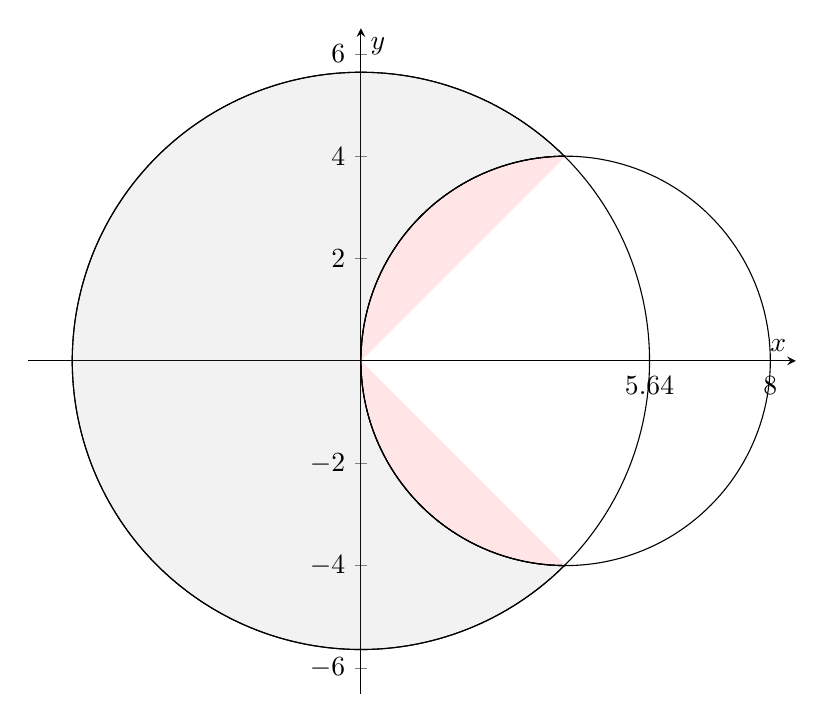
\begin{tikzpicture}
\begin{axis}[
x= 0.65 cm, y=0.65 cm,
 axis lines=middle,
  xmin=-6.5,xmax=8.5,ymin=-6.5,ymax=6.5,
  xtick={5.64,8},
  ytick distance = 2,
  xlabel=$x$,
  ylabel=$y$]
\addplot[domain=0:180,samples=5000,data cs=polar] (x,{8*cos(x)});
\addplot[domain=0:360,samples=500,data cs=polar] (x,{4*1.41});
\addplot[domain=45:90,name path = B,samples=300,data cs=polar] (x,{8*cos(x)});
\addplot[domain=45:90,name path = A,samples=300,data cs=polar] (x,{4*1.41});
\addplot[domain=90:180,name path = E,samples=300,data cs=polar] (x,{4*1.41});
\addplot[domain=90:180,name path = F,samples=300,data cs=polar] (x,{0});
\addplot[domain=180:270,name path = G,samples=300,data cs=polar] (x,{4*1.41});
\addplot[domain=180:270,name path = H,samples=300,data cs=polar] (x,{0});
\addplot[domain=90:135,name path = C,samples=300,data cs=polar] (x,{8*cos(x)});
\addplot[domain=270:315,name path = D,samples=300,data cs=polar] (x,{4*1.41});
\addplot[domain=45:90,name path = I,samples=300,data cs=polar] (x,{8*cos(x)});
\addplot[domain=45:90,name path = J,samples=300,data cs=polar] (x,{0});
\addplot[domain=90:135,name path = K,samples=300,data cs=polar] (x,{8*cos(x)});
\addplot[domain=270:315,name path = L,samples=300,data cs=polar] (x,{0});
\addplot[gray,opacity=0.1] fill between[of=B and A];
\addplot[red,opacity=0.1] fill between[of=J and I];
\addplot[red,opacity=0.1] fill between[of=K and L];
\addplot[gray,opacity=0.1] fill between[of=C and D];
\addplot[gray,opacity=0.1] fill between[of=E and F];
\addplot[gray,opacity=0.1] fill between[of=G and H];
\end{axis}
\end{tikzpicture}
	\end{center}
 Tinjau titik potongnya, yaitu 
 \begin{align*}
     4\sqrt{2} &= 8\cos\theta \\
     \cos\theta = \dfrac{1}{2}\sqrt{2}
 \end{align*}
 Didapat $\theta=\frac{\pi}{4},-\frac{\pi}{4}$. Selanjutnya, dapat dihitung luasannya, yaitu luasan lingkaran $r=4\sqrt{2}$ dengan $\theta$ dari $\frac{\pi}{4}$ sampai $\frac{7\pi}{4}$ dikurangi dengan luasan lingkaran $r=8\cos\theta$ dengan $\theta$ dari $\frac{\pi}{4}$ sampai $\frac{3\pi}{4}$.\\
 Karena kurvanya simetris, maka didapat luasannya adalah 
 \begingroup
 \allowdisplaybreaks
 \begin{align*}
     L &= 2\qty(\int_{\pi/4}^{\pi} \frac{1}{2}(4\sqrt{2})^2\dd \theta-\int_{\pi/4}^{\pi/2} \frac{1}{2}(8\cos\theta)^2\dd\theta)\\
     &=\int_{\pi/4}^{\pi} 32 \dd \theta -\int_{\pi/4}^{\pi/2}64\cos^2\theta\dd \theta\\
     &= 32\theta\big|_{\pi/4}^{\pi}- \int_{\pi/4}^{\pi/2} 64\qty(\frac{1+\cos 2\theta}{2})\dd \theta\\
     &= 32\pi-8\pi-32\qty(\theta +\frac{\sin 2\theta}{2})\big|_{\pi/4}^{\pi/2}\\
     &= 24\pi -32\qty(\frac{\pi}{2}-\frac{\pi}{4}+\frac{\sin(\pi)-\sin(\pi/2)}{2})\\
     &= 24\pi - 8\pi +16\\
     &= 16\pi+16 = 16(\pi+1).
 \end{align*}
 \endgroup
\end{enumerate}
\end{document}
